\documentclass{article}
\usepackage[T2A]{fontenc}
\usepackage[utf8]{inputenc}
\usepackage[russian]{babel}
\usepackage{graphicx}

\begin{document}

\section{Простая вставка}
Вот картинка, вставленная напрямую:
\begin{center}
    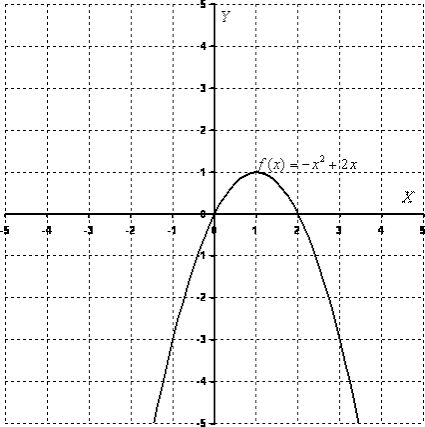
\includegraphics[width=0.5\textwidth]{1.png}
\end{center}

\section{Картинка с подписью и ссылкой}
На рисунке~\ref{fig:my_pic} показана картинка.
\begin{figure}[ht]
    \centering
    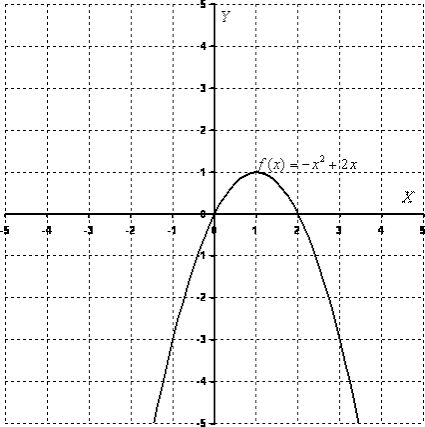
\includegraphics[width=0.5\textwidth]{1.png}
    \caption{Какая-то картинка}
    \label{fig:my_pic}
\end{figure}

\section{Размеры}
Картинка с фиксированной высотой повернутая на 45 градусов:
\begin{center}
    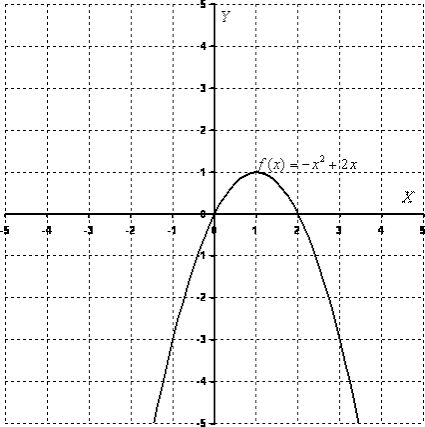
\includegraphics[angle=45, width=0.3\textwidth]{1.png}
\end{center}

\section{Размеры}
Картинка с фиксированной высотой повернутая на 45 градусов:
\begin{center}
    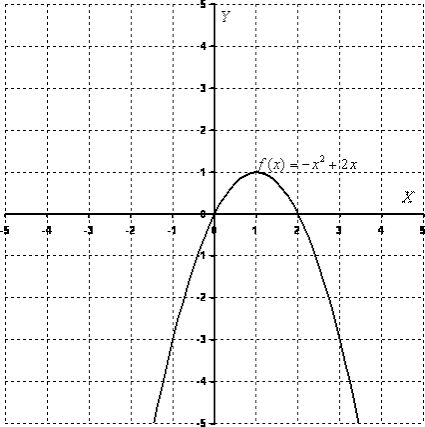
\includegraphics[angle=45, width=0.3\textwidth]{1.png}
\end{center}

\end{document}